\documentclass[12pt,letterpaper]{article}
\input{../../preamble}
\usepackage{fullpage}
\usepackage{multicol}
%\everymath{\displaystyle}

\begin{document}
\flushleft
\begin{multicols}{2}

%\begin{large}
\textbf{Math 2554 Exam 1: Limits ($\oint$2.1-3.1) \\
Fri 6 Feb 2015}
%\end{large}

%\hfill
\textbf{Name:  } \\

\vspace{1pc}
\underline{\hspace{43ex}} %KEY\hspace{17ex}} 
\\
\vspace{.5in}

\end{multicols}

\pagestyle{empty}

\flushleft

\begin{center}\LARGE Calculus I 

Exam 1 \end{center}

\vspace{1.5pc}
Please provide the following data:

\vspace{1.5pc}
Drill Instructor: \underline{\hspace{40ex}}

\vspace{1.5pc}
Drill Time: \underline{\hspace{40ex}}

\vspace{1.5pc}
Student ID or clicker \#: \underline{\hspace{40ex}}

%\vfill
\vspace{3pc}
{\bf Exam Instructions:} You have 50 minutes to complete this exam.  One $3\times 5$ inch notecard, one side only, is allowed.  No graphing calculators.  No programmable calculators.  No electronic devices except for the approved calculators (so no phones, iDevices, computers, etc).  If you finish early then you may leave, UNLESS there are less than 5 minutes of class left.  To prevent disruption, if you finish with less than 5 minutes of class remaining then please stay seated and quiet.

%\vspace{2pc}
\vfill
\textbf{Your signature below indicates that you have read this page and agree to follow the Academic Honesty Policies of the University of Arkansas.}  

\vspace{2pc}
Signature: {\bf (1 pt)} \underline{\hspace{91ex}}

%\vfill
\begin{flushright}\Large Good luck!\end{flushright}

\begin{enumerate}
\newpage

\item {\bf (3 pts ea)} Evaluate the following limits, analytically.  Write down justification for each answer.

\vspace{1pc}
\begin{enumerate}
\item $\displaystyle\lim_{x\to 0}x^2\cos x$

\vspace{14pc}
\item $\displaystyle\lim_{x\to -5}\pi$

\vspace{14pc}
\item $\displaystyle\lim_{x\to 0}\frac{x^3-5x^2}{x^2}$
\end{enumerate}

% % %
\newpage
\item {\bf (3 pts ea)} Suppose 
$\displaystyle\lim_{x\to 1}f(x)=8,\;\displaystyle\lim_{x\to 1}g(x)=3,\text{ and }\displaystyle\lim_{x\to 1}h(x)=2.$  
Compute the following limits and state the limit laws used (and why you are allowed to use them in that instance, if there is a caveat) to justify your computations.  If the limit does not exist then say so.

\vspace{1pc}
\begin{enumerate}
\item $\displaystyle\lim_{x\to 1}4f(x)$

\vspace{13pc}
\item $\displaystyle\lim_{x\to 1}\frac{f(x)g(x)}{h(x)}$

\vspace{13pc}
\item $\displaystyle\lim_{x\to 1}\sqrt[3]{f(x)g(x)+3}$
\end{enumerate}

% % %
\newpage
\item {\bf (3 pts ea)} Figure \ref{fig:epsDel} shows the piecewise linear function $f(x)$.  In each statement, determine the appropriate value of $\delta>0$.  If no such $\delta$ exists, say why. 
\begin{figure}[h]
\centering{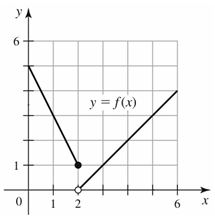
\includegraphics[scale=1.25]{Exam1epsDelpic}}
\caption{p. 117 \emph{Calculus: Early Transcendentals}, Briggs, et al.}
\label{fig:epsDel}
\end{figure}
	\begin{enumerate}
	\item $|f(x)-0|<2$ whenever $0<|x-2|<\delta$
	
	\vspace{6pc}
	\item $|f(x)-0|<1$ whenever $0<|x-2|<\delta$
	
	\vspace{6pc}
	\item $|f(x)-1|<2$ whenever $0<|x-2|<\delta$
	
	\vspace{6pc}
	\item $|f(x)-1|<1$ whenever $0<|x-2|<\delta$
	\end{enumerate}
	
% % %
\newpage
\item {\bf (12 pts ea)} For each function below,
\begin{itemize}
\item Determine the end behavior, including any horizontal asymptotes.  If there is no horizontal asymptote, then say so.   
\item Find the vertical asymptotes.  For each vertical asymptote $x=a$, evaluate $\displaystyle\lim_{x\to a^-}f(x)$ and $\displaystyle\lim_{x\to a^+}f(x)$. 
\end{itemize}

\vspace{1pc}
\begin{enumerate}
\item $f(x)=\displaystyle\frac{x^2-9}{x(x-3)}$

% % % 
\newpage
\item $f(x)=\displaystyle\frac{\sqrt{16x^4+64x^2}+x^2}{2x^2-4}$
\end{enumerate}

% % %
\newpage
\item \begin{enumerate}
	\item {\bf (7 pts)} Let $f(x)=x^2-5$.  Evaluate, analytically:
	\[\displaystyle\lim_{x\to 3}\frac{f(x)-f(3)}{x-3}\]

	\vspace{23pc}
	\item {\bf (3 pts)} Use your answer from (a) to write the equation of the tangent line to $f(x)$ at $x=3$.
	\end{enumerate}

% % %
\newpage
\item {\bf (2 pts ea)} Suppose $s(t)$ is the position of an object moving along a line at a time $t\geq 0$.  

\vspace{1pc}
\begin{enumerate}
\item Write the formula for the average velocity between the times $t=a$ and $t=b$.

\vspace{10pc} 
\item Write the formula for the instantaneous velocity at $t=a$.  
\end{enumerate}

\vspace{10pc}
\item {\bf (6 pts)} Write down the three conditions $f(x)$ must satisfy to be continuous at $a$ (a.k.a. the Continuity Checklist).
\end{enumerate}

% % %
\newpage
{\bf ChAlLeNgE pRoBlEm (0 pts):} Suppose a spaceship is traveling at velocity $v$, relative to an observer.  Say the length of the spaceship is $L_0$.  To the observer, the ship appears to have a smaller length, given by the Lorentz contraction formula:
\[\text{length to the observer}=L_0\sqrt{1-\frac{v^2}{c^2}},\]
where $c$ is the speed of light.
\begin{enumerate}[(a)]
\item If $v=0.5c$, i.e., the ship is traveling at half the speed of light, then how long does the ship look to the observer?

\vspace{12pc}
\item If the ship is traveling 75\% of the speed of light then how long does the ship look to the observer?

\vspace{12pc}
\item Compute $\displaystyle\lim_{v\to c^-}L_0\sqrt{1-\frac{v^2}{c^2}}$.  What is physically interesting about this limit?
\end{enumerate}
\end{document}


